\documentclass[a4paper,12pt]{article}
\usepackage[pdftex]{graphicx}
\usepackage[spanish]{babel}
\usepackage{ucs}
\usepackage[utf8x]{inputenc}
%\usepackage[T1]{fontenc}
\usepackage{times}
%\renewcommand{\familydefault}{phv}
\usepackage[sc]{mathpazo}
\usepackage[colorlinks=true,linkcolor=black, urlcolor=black, citecolor=blue]{hyperref}
%\linespread{1.5}
%\renewcommand{\baselinestretch}{1.5}
%%%%%%%%%%%%%%%%%%%%%
\fontsize{12}{12}\selectfont
\pretolerance=3000
\tolerance=3000
\title{\vspace*{4cm} 
\includegraphics[height=0.1\textheight]{utfsm.png}\\ \vspace*{0.2cm}
\tiny{SEDE JOSÉ MIGUEL CARRERA \\ VIÑA DEL MAR} \vspace*{2cm} \\ 
\Huge {Presentación Tema \\ Trabajo de Titulación} \\ \vspace*{0.5cm}
	 \Large{Técnico Universitario en Informática}}
\author{Bernardo Arancibia Araos
\and Sebastián Machuca Sáez}
\date{\today}

\marginparwidth 40pt
\marginparsep 10pt
%\topmargin 0pt
\headsep .5in
%\textheight 8.1in
%\textwidth 6in
\hoffset        -1.0in  % Seteo a 0 el margen izquierdo
\oddsidemargin   4cm    % Margen izquierdo (pag. impar)
%\oddsidemargin     0cm  % Ancho Legal 21,59cm
\evensidemargin  0.5cm  % Alto  Legal 35,56cm
\textwidth      15.5cm
\topmargin      -1.5cm
%\voffset           2cm  % Margen superior
\textheight       22cm
%\parindent      0em
%\parskip        2e

% Redefinir los macros utilizados para los pie de p�ginas para usar espaciamiento simple.
\long\def\@footnotetext#1{%
    \insert\footins{%
        \def\baselinestretch{1}\footnotesize
        \interlinepenalty\interfootnotelinepenalty 
        \splittopskip\footnotesep
        \splitmaxdepth \dp\strutbox \floatingpenalty \@MM
        \hsize\columnwidth \@parboxrestore
        \edef\@currentlabel{\csname p@footnote\endcsname\@thefnmark}\@makefntext
        {\rule{\z@}{\footnotesep}\ignorespaces#1\strut}%
    }%
}

\fontsize{12}{12}\selectfont
\linespread{1.5}

\begin{document}

\maketitle
\thispagestyle{empty} % No aparece el número de página en la portada
\newpage

\tableofcontents
\newpage

\section{Datos Generales}
\subsection{Identificación:}

  \begin{itemize}
   \item \textbf{Nombre:} \textbf{Bernardo Andrés Arancibia Araos} \\
         \textbf{Teléfono:} 09-86014468 \\ 
         \textbf{E-mail:} bernardo@kde.cl
  \end{itemize}
  \begin{itemize}
   \item \textbf{Nombre:} \textbf{Sebastián Alonso Machuca Sáez} \\
         \textbf{Teléfono:} 09-87706855 \\
         \textbf{E-mail:} sebastian.machuca@alumnos.usm.cl
  \end{itemize}

\subsection{Nombre del Tema:}
   ``Administración y Vitrina Online para negocios de barrio''

\subsection{Empresa o Institución:}
  \begin{description}
   \item [Nombre Empresa:] \emph{Provisiones Frutas y Verduras ``Chusmisa''} (Pyme)
   \item [Nombre Supervisor:] Bernardo Arancibia Quiroz
   \item [Teléfono:]{ 032-2856979 / 032-2851359}
  \end{description}

\subsection{Ambiente Computacional}
  \begin{description}
   \item [Arquitectura:] PC (i686)
   \item [Sistema Operativo:] GNU/Linux
   \item [Lenguaje de Programación: ] Qt Framework, Ruby on Rails
   \item [Herramientas: ] Mysql \footnote{Motor de Base de Datos}, GIT \footnote{Herramientas de Control de 
    Versiones de Software}, PivotalTracker \footnote{Herramienta para gestionar \emph{bugs} y \emph{features}}
  \end{description}

\subsection{Objetivos del Tema:}
  \begin{itemize}
   \item Realizar un \emph{pack} de aplicaciones que permitan introducir a pequeños negocios de barrio (abarrotes) en el 
         uso de las nuevas tecnologías de la información, optimizando y automatizando las tareas que éstos realizan diariamente.

   \item Que las aplicaciones sean fáciles y rápidas de utilizar, para así no afectar el tiempo de atención de un cliente.

   \item Lograr que la interacción \emph{cliente}-\emph{negocio} sea óptima y más organizada.
  \end{itemize}

\pagebreak

\section{Descripción del Tema:}
\subsection{Descripción de la situación actual:} %%%%%%%%%%%% REVISAR
    Hoy en día los pequeños negocios se ven ajenos a la automatización de sus tareas, debido al alto costo 
  que esto significa para sus dueños; los negocios deben sacar cuentas, obtener balances, y sobretodo ofrecer 
  un servicio rápido, seguro y fácil de usar, que permita sacar ventajas para mejorar la competencia en el área.

    Los usuarios o consumidores de los pequeños negocios cada vez son menos, prefieren las grandes tiendas 
  para satisfacer sus necesidades, ya que estas tiendas ofrecen diversas facilidades para acceder a su 
  mercadería, hablamos de Catálogos Online, compras Online, entre otros. 

    Según la última encuesta de la Subtel \cite{subtel} (dada a conocer a inicios de febrero del presente año) 4 de cada 10 
  hogares posee conexión a Internet, si tomamos en cuenta el año 2008, esta cifra se reduce a 2 de cada 10. Con estos 
  datos se puede demostrar los puntos anteriormente mencionados, Internet se ha transformado en una herramienta
  indispensable y del diario vivir para mucho de los chilenos.

\subsection{Problemas detectados:}
  \begin{enumerate}
   \item \textbf{Baja automatización en tareas administrativas:} Los dueños de pequeños negocios 
   se ven constantemente obligados a realizar sus cálculos, estadísticas y balances de manera manual. 
   Esto requiere mucha concentración y trabajo por parte de los dueños ya que un número mal anotado es un 
   balance mal hecho, sin contar lo tedioso que puede ser para una persona que trabaja sola
   y no posee ayudantes.

\newpage

  \item \textbf{Poca participación de herramientas digitales en los pequeños negocios:} Los pequeños
   negocios corren con desventaja con respecto a las grandes empresas debido a su poca participación en la \emph{web} 
   y el uso de aplicaciones que facilitan el acceso a sus productos, todo esto se debe al alto costo que estas 
   herramientas necesitan para poder implementarse, no sólo el costo de implementación sino que también por 
   el costo de las licencias de las aplicaciones genéricas que existen actualmente en el mercado, es aquí donde
   entra fuertemente la necesidad de hacer uso de herramientas de Software Libre.
  
  \item \textbf{Centralización de la información en una sola persona:} La gran mayoría de estos negocios
   son administrados por su dueño y atendidos por otra persona, quien debe mantener en su memoria los precios
   actualizados de cada producto. Muchas veces el dueño no tiene tiempo de hacer una
   lista con todos los precios, por lo cual la persona que está vendiendo no va a saber el precio actual de un 
   producto a menos que pregunte todos los días por éste.

   Generalmente el dueño es quien completa el \emph{Libro de Compra Venta}, el \emph{Cuaderno de Ventas inferiores a} 
  \$180 y el cálculo en el porcentaje y precio actual de venta, además del \emph{Resumen de Ventas Diarias}.
  \end{enumerate}

\newpage

\subsection{Descripción del sistema propuesto:}

 \subsubsection{Objetivos específicos del sistema propuesto:}
  Realizar dos aplicaciones con dos \emph{frameworks} diferentes, orientados específicamente para el desarrollo de las tareas
  que se necesitarán. 

  La primera aplicación será de tipo \emph{``desktop``} y estará destinada para el manejo de las ventas
  diarias que se realizan, junto con algunas otras funcionalidades que se requieren en un negocio de barrio.

  La segunda aplicación será de tipo \emph{``web''} y consiste en una página \emph{web} que contendrá los datos de los productos que
  se venden en el negocio, sus precios, disponibilidad, etc.
  
  La plataforma \emph{web} permitirá mantener a los clientes actualizados con los nuevos productos y sus precios, además mantener un 
  contacto más cercano y eficiente al momento de obtener información de su proveedor de abarrotes. 
  La idea principal no es vender por Internet, ya que para este tipo de negocio de barrio sería una forma muy complicada de
  administrar el dinero (Tarjeta de Crédito, Cuenta Bancaria), sin contar que tendría que realizar despachos a domicilio
  de los mismos productos. 
  Nuestra principal labor es hacer más fácil las tareas del vendedor y dueño del negocio, por lo que nos enfocaremos a 
  que sea un servicio de \emph{``Vitrina Online y Gestión de Pedidos''}. Esta aplicación se conectará a la base de datos 
  de productos disponibles compartida con la aplicación \emph{``desktop''}.

\newpage

\subsubsection{Funcionalidad del sistema:}

  \begin{itemize}
   \item \textbf{Aplicación Administrativa:} 
    Aplicación escrita en el lenguaje \emph{QT} \cite{qtweb}, un símil del lenguaje
    \emph{Visual Basic}, es decir orientado al evento, pero desarrollado para ser multiplataforma. 
    Este lenguaje hace uso de sus propias características junto con funciones y argumentos del lenguaje C++.

    La principal tarea de este programa, es ser ejecutada en el escritorio del vendedor al momento de vender un
    determinado producto y que los datos de las ventas sean respaldadas en una base de datos. Cada producto se debe
    ingresar vía teclado, y el programa tendrá la funcionalidad de ir autocompletando el nombre del producto y mostrar
    los diferentes subproductos para cada tipo (ejemplo: coca-cola 1 litro, coca-cola 3 litros; arroz 1 Kg, arroz 1/2 Kg).

    Todas las modificaciones en los precios de los productos y stock serán realizados en esta aplicación, cuyos datos 
    finalmente se volcarán en la base de datos destinada para guardar toda la información necesaria.

    Se crearán cuentas de \emph{administrador} y \emph{vendedor} para así mantener una jerarquía que permita limitar
    a quienes realicen cambios en los precios de los productos. \\
    
    
    \textbf{Funciones específicas a realizar:}
      \begin{enumerate}
       \item \textbf{Autentificación: }Cuentas para gestionar el programa. La cuenta \emph{Administrador} posee la facultad de modificar los
			     atributos de los productos y a la vez la facultad de crear nuevos productos y eliminarlos.

                             La cuenta \emph{Vendedor} permite gestionar las ventas y todas las demás funciones que esto involucra, 
			     exceptuando la modificación de los productos.

       \newpage

       \item \textbf{Ingresar Nuevo Producto: }Se ingresa un nuevo producto a la tabla \emph{Productos} con sus correspondientes atributos.

       \item \textbf{Eliminar Un Producto Existente: }Se elimina un determinado producto de la tabla \emph{Productos} previamente validada su
                                                      existencia en dicha tabla.

       \item \textbf{Modificar Un Producto Existente: }Se modificarán los atributos del producto especificado, previamente validado.

       \item \textbf{Ingresar Venta: }Luego de ser cancelada una compra por un cliente, se desea ingresar la venta en la tabla \emph{Ventas}
				      en la Base de Datos.
       \item \textbf{Eliminar Venta: }Existiendo la posibilidad de que un cliente se arrepienta de una compra ya ingresada en el sistema,
                                      se debe eliminar una venta de la tabla \emph{Venta} y su respectivo detalle en la tabla \emph{Detalle\_Venta}
                                      en la Base de Datos.
       \item \textbf{Modificar Venta: }Producto de algun error, se desean modificar los atributos de una respectiva venta realizada.

       \item \textbf{Ingresar Cliente: }Se registra un nuevo cliente, indicando sus datos personales, atributos como es el caso de
					\emph{estado}, el cual indica si un cliente es moroso o tiene su cuenta al día.

       \item \textbf{Eliminar Cliente: }Se elimina un cliente que no desea seguir registrado.

       \item \textbf{Modificar Cliente: }Se actualizan los datos de un cliente.

       \item \textbf{Ingresar Venta a Fiado: }Teniendo un cliente registrado, se le asigna una venta sin cancelar en la tabla
					      \emph{Fiados}, para su posterior pago, esto además modifica el campo \emph{estado} en la tabla
					      \emph{Venta} indicando si la venta ha sido pagada o se ha agregado a la tabla \emph{Fiados}.

       \item \textbf{Modificar Venta a Fiado: }En caso de error existe la posibilidad de modificar una venta en la tabla \emph{Fiados}.

       \item \textbf{Consultar Producto: }Se desea buscar un determinado producto por su nombre en la tabla \emph{Productos}.

       \item \textbf{Consultar Venta: }Se desea buscar una determinada venta realizada por su fecha.

       \item \textbf{Consultar Venta Fiado: }Se desea buscar una determinada venta fiada a partir de un cliente.

       \item \textbf{Consultar Cliente: }Se desea buscar un determinado cliente a partir de su nombre.
      
       \item \textbf{Consultar Pedidos: }Ver todos los pedidos efectuados a través de la plataforma \emph{web}.

       \item \textbf{Agregar Usuario:} Se ingresa un nuevo usuario a la tabla \emph{Usuarios}, además se debe
				      indicar el tipo de usuario correspondiente (Administrador, Vendedor),
				      guardándose este valor en el atributo \emph{tipo\_usuario} en la tabla
				      \emph{Usuarios}.

       \item \textbf{Eliminar Usuario:} Se elimina un usuario con sus respectivos atributos de la tabla \emph{Usuarios}.


       \item \textbf{Modificar Usuario:} Se actualizan los datos de un usuario.

       \item \textbf{Ingresar Categoría:} Se ingresa una nueva categoría a la tabla \emph{Categorias} para poder clasificar los productos, 
					  en el caso de que el producto no tenga categoría quedará en calidad de ``Sin Categoría''.

       \item \textbf{Modificar Categoría:} Se actualizan los datos de una categoría.

       \item \textbf{Eliminar Categoría:} Se desea eliminar una categoría con sus respectivos atributos de la tabla \emph{Categorias}.


      \end{enumerate}
     
  \newpage    
      
   \item \textbf{Aplicación de Vitrina Online:}
    Aplicación escrita bajo \emph{Ruby on Rails} \cite{railsweb} , framework destinado a la creación 
    de aplicaciones web. 

    La \emph{``Vitrina Online``} no es más que un catálogo que permite excibir los productos que en la tienda se encuentran, junto
    con sus precios y su disponibilidad. De esta forma, el negocio además de poseer un sitio web personal, tendrá este
    catálogo, junto con la posibilidad de compartir mensajes y pedidos con sus clientes. La principal funcionalidad de
    esta aplicación se basa en que hace uso de la base de datos de productos para obtener la información a mostrar,
    base de datos compartida con la aplicación Administrativa escrita en \emph{Qt}. \\

    \textbf{Funciones específicas a realizar:}
    \begin{enumerate}
     \item \textbf{Autentificación: }Para poder realizar un pedido, un cliente debe estar registrado en la tabla \emph{Clientes} de la base de 
			   datos. Esta autenticación es proporcionada por una aplicación de la plataforma \emph{web}. El registro de los 
			   clientes será efectuado de forma presencial en el negocio, por medio de la aplicación de escritorio.

     \item \textbf{Ingresar Pedido: }El cliente desea reservar una determinada lista de productos. Esta función será proporcionada
			            por una aplicación \emph{web} del tipo \emph{carrito de compras}, juntando cada producto como un
				    ítem y adjuntando su cantidad. La idea de esta aplicación es enviar este pedido a la tabla
                                    \emph{Pedidos} para reservar un determinado producto. Debe quedar en claro que esta funcionalidad 
				    no involucra el manejo de dinero (tarjetas de crédito, débito, etc.), sólo involucra el registro 
				    de los pedidos para luego ser entregados físicamente en el mismo negocio y así finalizar la transacción.

     \newpage

     \item \textbf{Modificar Pedido: } Un cliente puede modificar un pedido, siempre y cuando este pedido no sea recepcionado todavía por un 
				      vendedor (\emph{estado\_pedido}). De esta forma, si el cliente comete un error en su pedido, o desea adjuntar nuevos productos 
				      a este pedido, podrá realizar sus modificaciones. Si se cometen errores luego de recepcionado el pedido, 
				      el cliente debe comunicarse vía telefónica o presencial con el vendedor.

     \item \textbf{Consultar Producto por Nombre:} Se desea buscar un producto ordenado por su respectivo nombre o marca.

     \item \textbf{Consultar Producto por Categoría: } Se desea buscar un producto ordenado por categoría.


    \end{enumerate}


  \end{itemize}

\newpage

\subsubsection{Entradas y Salidas del Sistema:}
\begin{itemize}
 \item \textbf{Entradas:} \\ \\
     \textbf{Datos Ingresados Por Teclado:}
     \begin{enumerate}
      \item Atributos necesarios para el registro de un nuevo usuario.
      \item Atributos necesarios para el registro de un nuevo cliente.
      \item Atributos de un nuevo producto.
      \item Atributos de una venta efectuada.
      \item Atributos de un nuevo pedido.
     \end{enumerate}


 \item \textbf{Salidas:}
     \begin{enumerate}
       \item \textbf{Listado de Clientes:} Se listan todos los clientes registrados hasta la fecha.

       \item \textbf{Listado de Usuarios:} Se listan los usuarios ingresados en el sistema.

       \item \textbf{Listado de Ventas:} Se listan todas las ventas efectuadas y su detalle correspondiente en una determinada fecha.

       \item \textbf{Listado de Pedidos}: Se listan todos los pedidos realizados en una determinada fecha para su posterior preparación.

       \item \textbf{Listado de Productos:} Se Listan todos los productos disponibles a la venta con sus respectivas características.
       
       \item \textbf{Listado por Categoría: } Se Listan todos los productos disponibles a la venta ordenado por categoría.

     \end{enumerate}
 
       
\end{itemize}

\newpage

\subsubsection{Entidades de Información:}

\textbf{Modelo Relacional Propuesto:}

\begin{figure}[!ht]
    \begin{center}
	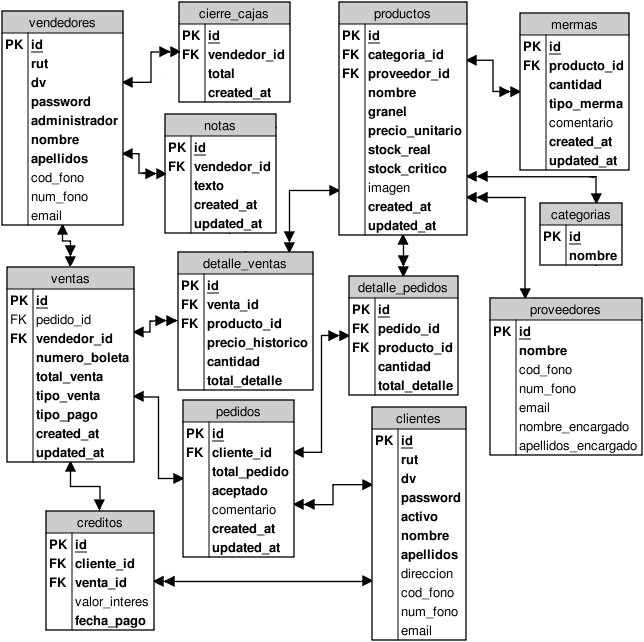
\includegraphics[width=1.0\textwidth]{docs/modelo_relacional.png}
    \end{center}
    \caption{Vista preliminar de las tablas a utilizar. A medida que se vaya construyendo el proyecto
             se añadirán nuevas tablas y argumentos.
	     La tabla \emph{Usuarios} podría variar en el desarrollo del proyecto a una tabla \emph{Vendedores}, 
	     para así administrar las ventas que cada vendedor realizó.}
\end{figure}

\newpage

\renewcommand{\refname}{\section{Referencias}}
\begin{thebibliography}{10}
 \bibitem{gitrepoweb}{\textbf{Repositorio GIT del proyecto}} \\ \url{http://github.com/trabajo-titulo/trabajo-de-titulo}
 \bibitem{pivotalweb}{\textbf{Pivotal Tracker}} \\ \url{http://www.pivotaltracker.com/}
 \bibitem{qtweb}{\textbf{Nokia Qt Framework}} \\ \url{http://qt.nokia.com/products}
 \bibitem{railsweb}{\textbf{Ruby on Rails}} \\ \url{http://rubyornrails.org/}
 \bibitem{subtel}{\textbf{Subsecretaría de Telecomunicaciones de Chile}} \\ \url{http://www.subtel.cl}
\end{thebibliography}

\end{document}
